%------------------
%	PRZEWODNIK PO UBUNTU 14.04 LTS TRUSTY THAR
%	
%
%	Autorzy:
%		1. Piotr "Dwimenor Vali" Sochocki, dwimeron@gmail.com
%
%	Licencja:
%		Creative Commons
%		Uznanie autorstwa-Uzycie niekomercyjne-Na tych samych warunkach 3.0 Polska
%		CC BY-NC-SA 3.0 PL
%		http://creativecommons.org/licenses/by-nc-sa/3.0/pl/
%------------------


%------------------
%	PREAMBUŁA
%------------------

% klasa mwart autorstwa Marcina Wolińskiego
% http://marcinwolinski.pl/mwcls.html
% pakiet: texlive-lang-polish
\documentclass[a4paper,11pt,oneside]{mwart}

% orientacja pozioma, marginesy
\usepackage[landscape, margin=0.5in]{geometry}

% interlinia (1.6 = półtora linni odstępu wg. nomenklatury Worda/Writera)
\linespread{1.6}

% Odległosć między akapitami
\setlength{\parskip}{0.2cm}

% Język polski, polfonty
\usepackage[OT4]{polski}
\usepackage[utf8]{inputenc}

% dzielenie wierszy
\brokenpenalty=1000
\clubpenalty=1000
\widowpenalty=1000

% Obrazki
\usepackage{graphicx}
\usepackage{wrapfig}

% linki, URL
\usepackage[urlcolor=blue, colorlinks=true]{hyperref} 

% Dwie kolumny w spisie treści
\usepackage[toc]{multitoc}

% Jako, że nie bawimy się w rozdziały, sekcja i podsekcja są podstawowymi jednostmaki podziału dokumentu.
% Poniższa komenda wymusza numerowanie sekcji od "1" zamiast od "0"
\renewcommand*\thesection{\arabic{section}}

% Gwizadka zamiast myślnika jak znak kolejnego punktu listy.
\renewcommand{\labelitemi}{$\star$}

% Oficjalne kolory Ubuntu
% http://design.ubuntu.com/brand/colour-palette
\usepackage{xcolor}
\definecolor{ubuntu_orange}{RGB}{221,72,20}

%------------------
%	STRUKTURA DOKUMENTU
%------------------

\begin{document}

\thispagestyle{empty}

%-----------------
%	TYTUŁ
%-----------------

\colorbox{ubuntu_orange}{
	\parbox[t]{1.0\linewidth}{
		\centering \fontsize{40pt}{70pt}\selectfont
		\vspace*{0.7cm}
		
		\hfill Przewodnik po\\
		\hfill Ubuntu 14.04 LTS\\
		\hfill Trusty Thar\par
		
		\vspace*{0.7cm}
	}
}

\vfill

%-----------------
%	AUTOR
%-----------------

{
	\centering
	\large 
	\hfill Zespół \href{http://www.ubuntu.pl}{Ubuntu.pl} \\
}
\clearpage

\tableofcontents
\clearpage
\section{Wstęp}
	\noindent Witaj w \textcolor{ubuntu_orange}{Przewodniku po Ubuntu Linux 14.04 Trusty Thar!}

Niniejszy dokument pomoże ci zainstalować oraz skonfigurować system operacyjny Ubuntu. Przewodnik obejmuje każdy etap procesu zmiany systemu, od przygotowania twoich plików i ustawień po instalowanie oraz używanie twojej świeżo zainstalowanej kopii Ubuntu.

Przewodnik ten został napisany z myślą o osobach nieposiadających wiedzy technicznej, a większość terminów technicznych opatrzono stosownymi objaśnieniami. Przewodnik zadaje także kłam mitowi, że użytkowanie Linuksa wiąże się z koniecznością wpisywania niezrozumiałych komend w konsoli. Cały tekst został przygotowany z myślą o wykorzystaniu graficznych narzędzi dostarczanych wraz z systemem.

Mamy nadzieję, że czytając ten przewodnik bezproblemowo zainstalujesz Ubuntu na swoim komputerze i będziesz zadowolony mogąc korzystać z darmowego oraz otwartego systemu operacyjnego.\\
Wersja Ubuntu, która została opisana w tym poradniku, nosi nazwę Ubuntu GNU/Linux 14.04 LTS Trusty Thar, co oznacza:
\begin{itemize}
\item \textcolor{ubuntu_orange}{Ubuntu} ---  nazwa całej serii systemów operacyjnych wydawanych przez firmę Canonical.
\item \textcolor{ubuntu_orange}{GNU/Linux} --- system bazuje na jądrze Linuksa i wykorzystuje oprogramowanie GNU.
\item \textcolor{ubuntu_orange}{14.04} --- jest to wersja z kwietnia (04) 2014 roku.
\item \textcolor{ubuntu_orange}{LTS} --- jest to wersja o przedłużonym wsparciu technicznym, a poprawki będą wydawane do 2019 roku).
\item \textcolor{ubuntu_orange}{Trusty Tahr} --- nazwa kodowa tego wydania.
\end{itemize}
	\subsection{O Ubuntu}
		Ubuntu jest kompletnym systemem operacyjnym utrzymywanym i rozwijanym przez firmę Canonical. Pierwsza jego wersja ukazała się w 2004 roku, a w ciągu14 lat system ten zdobył rzesze fanów. Ubuntu wraz ze swoimi odmianami jest najpopularniejszą na świecie dystrybucją Linuksa. Samo słowo Ubuntu w języku afrykańskiego plemienia Zulusów oznacza ”człowieczeństwo wobec innych”, w kontekście systemu operacyjnego tłumaczone jest jednak jako ”Linux dla ludzi”.

Ideą systemu Ubuntu jest dostarczenie użytkownikowi kompletnego systemu operacyjnego, zawierającego wszystkie elementy niezbędne do codziennej pracy, a jednocześnie umożliwiające posiadaczowi komputera swobodne korzystanie z systemu i modyfikowanie poszczególnych jego elementów. Wybierając Ubuntu nie musisz się zastanawiać nad tym, czy twój procesor nie ma przypadkiem zbyt dużej liczby rdzeni, co w przypadku korzystania z systemu komercyjnego mogłoby wymagać zakupu innej licencji. Nie musisz się również przejmować tym, że w firmie masz dziesięć komputerów, a twoja licencja na pakiet biurowy pozwala na instalację jedynie na sześciu stanowiskach. Jeśli chodzi o to, jak i do czego wykorzystasz system i oprogramowanie, wszystko zależy wyłącznie od ciebie.

Ubuntu pozwala także na daleko idące modyfikacje systemu - kod źródłowy jest otwarty, co pozwala każdemu na głębokie ingerencje w system. Choć powyższe zdanie może brzmieć groźnie, nie ma powodów do obaw - Ubuntu nie jest przeznaczone tylko dla doświadczonych komputerowych “magików”. Każdy może dowolnie dostosować swój system do własnych potrzeb i upodobań, czy to metodą zrób to sam, czy też poprzez odwołanie się do zasobów oferowanych przez społeczność.

Skoro poruszyliśmy już ten temat - społeczność skupiona wokół Ubuntu jest najważniejszą siłą napędzającą rozwój tej dystrybucji. Dodatki zmieniające wygląd systemu, nowe ikony i grafiki, dźwięki systemowe, tłumaczenia, całe zestawy oprogramowania - wszystkie te elementy (oraz wiele innych rzeczy) czekają, aż zdecydujesz się z nich skorzystać.
\clearpage

	\subsection{Dlaczego warto zmienić system na Ubuntu?}
		\subsubsection{Jest stabilny}
Ubuntu bazuje na słynącym ze stabilności systemie Debian GNU/Linux. Zapomnij o błędach krytycznych i zawieszaniu się komputera, przyzwyczaj się natomiast do niezawodnego systemu, który po prostu działa. Standardy jakości Debiana są bardzo wysokie i do ostatecznej wersji tego systemu nie trafi nic, co mogłoby nagle się popsuć. Jeśli instalujesz pod Ubuntu jakąś aplikację, możesz mieć pewność, że została już ona przetestowana przez tysiące ludzi rozsianych po całym świecie.
\begin{itemize}
\item Debian GNU/Linux jest tak stabilny, że pod jego kontrolą pracują najważniejsze systemy komputerowe świata, wliczając w to superkomputery oraz serwery wielkich portali internetowych.
\item Poprawki eliminujące znalezione błędy trafiają do systemu na bieżąco i nie trzeba na nie czekać miesiącami.
\item Każdy może zgłaszać znalezione błędy i śledzić proces ich naprawiania.
\end{itemize}
\subsubsection{Jest bezpieczny}
Ubuntu prezentuje zupełnie inne podejście do zagadnienia bezpieczeństwa niż inne systemy operacyjne. Tutaj bezpieczeństwo wynika z samej konstrukcji systemu,nie jest natomiast rezultatem nakładania na niego kolejnych łatek i dodatkowych warstw ochronnych. System jest bezpieczny, ponieważ likwiduje się przyczynę ewentualnych problemów, a nie leczy objawy. Co więcej, błędy, które mogłyby mieć negatywny wpływ na bezpieczeństwo użytkownika, naprawiane są niemal natychmiast. Nierzadko zdarza się, że od momentu wykrycia luki do chwili instalacji stosownej poprawki na milionach komputerów mija mniej niż doba.
\begin{itemize}
\item Ponieważ różne dystrybucje Linuksa cechują się wysokim poziomem bezpieczeństwa, to właśnie te systemy operacyjne można znaleźć na bardzo wielu serwerach sieciowych.
\item Wprowadzanie poważniejszych zmian w systemie pociąga za sobą konieczność podania hasła administratora. Ubuntu jest dzięki temu zabezpieczone zarówno przed potencjalnymi intruzami, jak i przed przypadkowym naruszeniem zasad bezpieczeństwa przez samego użytkownika.
\end{itemize}
\subsubsection{Jest łatwy w użyciu}
Słowo Ubuntu tłumaczy się jako ”\textit{człowieczeństwo wobec innych}”,  także “Linux dla ludzi”. Użytkowane przez ciebie programy zostały zaprojektowane w taki sposób, by nie były bardziej skomplikowane, niż to konieczne. To wcale nie znaczy, że Ubuntu ma ograniczone możliwości czy brakuje mocy - wręcz przeciwnie, pulpit Ubuntu jest pełen innowacyjnych funkcji.
\begin{itemize}
\item Komunikaty są sformułowane w jednoznaczny sposób, więc będziesz potrzebował przeczytać je tylko raz.
\item Aplikacje są ułożone tak, aby było je łatwo znaleźć.
\item Programy mają schludny i nowoczesny interfejs, dzięki któremu łatwiej będzie ci skupić się na czekających cię zadaniach.
\end{itemize}
\subsubsection{Jest międzynarodowy}
Nieważne gdzie mieszkasz i w jakim języku mówisz - możesz być pewien, że Ubuntu będzie się komunikowało z każdym użytkownikiem w najbardziej zrozumiały dla niego sposób. Dostęp do różnych wersji językowych jest bardzo prosty, a zmiana języka systemu ogranicza się do kilku kliknięć.
Oprócz  tłumaczeń obejmujących między innymi komunikaty systemowe, interfejs użytkownika czy menu poszczególnych aplikacji, Ubuntu oferuje również pełny wybór zestawów znaków i metod wprowadzania tekstu, możesz więc porozumiewać się ze swoim komputerem w dowolnie wybranym języku.
\begin{itemize}
\item Tłumaczenia są tworzone przez ochotników z całego świata.
\item Możesz samemu zaangażować się w tłumaczenia, korzystając z internetowej usługi Launchpad.
\item Aplikacja “Języki” pozwala szybko i wygodnie instalować nowe paczki językowe .
\end{itemize}
\subsubsection{Jest dostępny}
Świeżo zainstalowane Ubuntu wyposażone jest w szereg narzędzi poprawiających łatwość dostępu - lupę, program czytający informacje pojawiające się na ekranie oraz klawiaturę ekranową. Projekt Ubuntu posiada Zespół Dostępności, który zajmuje się wyłącznie tym, aby Ubuntu stawało się coraz bardziej dostępne dla każdego.
\begin{itemize}
\item Użytkownik może korzystać z ułatwień dostępu przez cały czas - od procesu instalacji począwszy, na codziennym użytkowaniu skończywszy.
\end{itemize}
\subsubsection{Jest wolny}
Ubuntu jest wolne i otwarte. Za instalację i użytkowanie tego systemu operacyjnego nigdy nie będziesz musiał zapłacić ani grosza. Nikt nie zabroni Ci również  modyfikowania, używania i rozprowadzania aplikacji wchodzących w skład Ubuntu. Nie musisz się zastanawiać nad tym, czy możesz wykorzystywać dany program, czy też jego licencja pozwala na przykład jedynie na ściśle określone zastosowania. W przypadku korzystania z Ubuntu nie ma takich ograniczeń - dysponujesz całkowitą wolnością w kwestii wykorzystywania i modyfikowania systemu oraz zawartego w nim oprogramowania.
Co więcej, zachęcamy cię do takiego postępowania! To oznacza, że zaoszczędzisz na oprogramowaniu, ale to nie wszystko - pamiętaj także, że jest ono całkowicie transparentne i otwarte na analizę. To pozwala szybciej wykrywać problemy związane z bezpieczeństwem, uniemożliwia ukrywanie przed niczego nieświadomym użytkownikiem przykrych niespodzianek, a na dodatek masz możliwość samodzielnego  dokonywania zmian w Ubuntu.
\begin{itemize}
\item Jeśli tylko posiadasz odpowiednią wiedzę techniczną, możesz samemu modyfikować swoje ulubione aplikacje.
\item Ubuntu może używać absolutnie każdy.
\end{itemize}
\subsubsection{Jest społecznościowy}
Społeczność to opoka, na której opiera się Ubuntu. Bez owej społeczności Ubuntu nie byłoby światowej klasy systemem operacyjnym, jakim jest w 2014 roku. Społeczność jest nierozłącznie związana z sukcesem Ubuntu i to właśnie ona zajmuje się wieloma rzeczami, od dostarczania tłumaczeń, testowania nowych wydań i zapewniani wsparcia, aż po pisanie nowego oprogramowania i rozwiązywanie problemów,  Każdy może pomóc w takim zakresie, w jakim potrafi i ma ochotę. Również i ty możesz pomóc kształtować kierunek rozwoju Ubuntu i ulepszać oprogramowanie dla ludzi z całego świata.
\begin{itemize}
\item Każdy może wnieść swój wkład w rozwój Ubuntu.
\item Ubuntu skupia ludzi posiadających bardzo różne zainteresowania. Programiści nie są jedynymi wybrańcami, którzy mają szansę zobaczyć efekty swojej pracy na milionach komputerów. Takie same możliwości mają graficy tworzacy tapety, muzycy komponujący dźwięki systemowe, designerzy projektujący ikony i zajmujący się wyglądem aplikacji, tłumacze dbający o to, by Ubuntu było dostępne w tylu językach, a także wiele, wiele innych osób.
\item Kodeks Postępowania Ubuntu i Rada Społeczności pomaga przewodzić społeczności i zapewnia każdemu możliwość przedstawienia swoich racji.
\end{itemize}
\clearpage

\section{Instalacja}
	\subsection{Pobieranie obrazu systemu}
		%TODO zweryfikować ten dokument jak już zaktualizują ubuntu.com
%obrazek
%linki
%rozmiar obrazów instalacyjnych
\begin{center}
	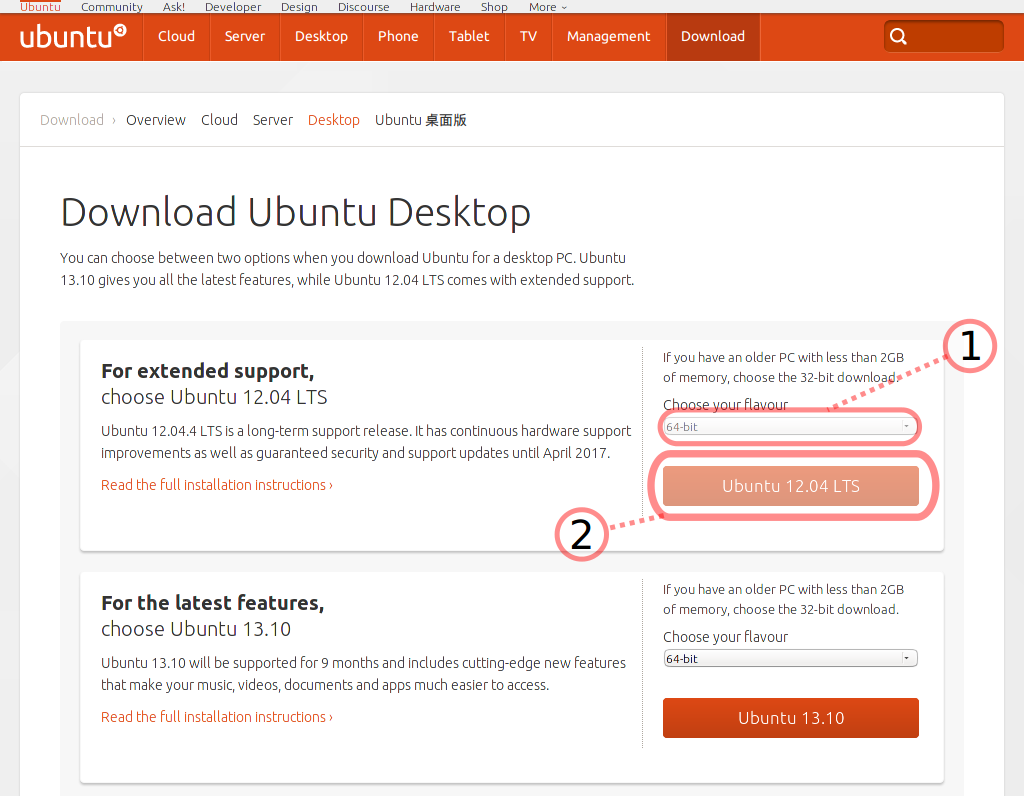
\includegraphics[width=\linewidth]{images/instalacja_pobieranie_obrazu.png}
\end{center}

Pierwszym etapem instalacji systemu jest pobranie instalatora. W tym celu udaj się na stronę \href{http://www.ubuntu.com/download/desktop}{ubuntu.com} i z górnego paska wybierz \textcolor{ubuntu_orange}{Download} a następnie \textcolor{ubuntu_orange}{Desktop}
\begin{enumerate}[label=\protect\circled{\arabic*}]
\item To pole pozwali ci wybrać pomiędzy 32- a 64-bitową wersją systemu. Domyślnie wybrana jest opcja 64 bitowa.
\item Kliknij na ten przycisk aby przejść dalej.
\end{enumerate}

Na kolejnym ekranie będziesz mieć możliwość przekazania dotacji na rzecz Ubuntu. W tym momencie nas to nie interesuje. Przesuń stronę w dół i kliknij na \textcolor{ubuntu_orange}{Not now, take me to the download}. Zostaniesz przeniesiony na kolejną stronę, a po kilku sekundach rozpocznie się pobieranie obrazu systemu.

Jeżeli twój komputer został wyprodukowany nie dawnej niż 5 lat temu, wersja 64-bitowa będzie na pewno odpowiednia. Jeżeli masz mniej niż 2 GB RAM-u, wybierz wariant 32-bitowy. Niezależnie od tego jaką wersję wybierzesz, i tak będziesz mieć dostęp do takiego samego zestawu oprogramowania. Wariant 64-bitowy jest lepiej dopasowany do nowoczesnych systemów, jeżeli jednak masz jakiekolwiek wątpliwości, wybierz wersję 32-bitową. Będzie ona działać także na 64-bitowym komputerze, choć nie będzie wykorzystywać wszystkich jego możliwości.
Jeżeli twoja płyta główna kontrolowana jest przez UEFI, musisz wybrać system 64-bitowy.
Linki do pobierania bezpośredniego:
\begin{itemize}
\item \href{http://www.ubuntu.com/start-download?distro=desktop&bits=64&release=lts}{Wersja 64 bitowa (733 megabajtów).}
\item \href{http://www.ubuntu.com/start-download?distro=desktop&bits=32&release=lts}{Wersja 32 bitowa (731 megabajtów).}
\end{itemize}
	\subsection{Nagrywanie pobranego obrazu}
		Po zakończeniu pobierania obrazu instalatora należy nagrać go na zewnętrzny nośnik i uruchomić komputer z tego nośnika. Najlepszym rozwiązaniem jest użycie klucza usb (pendriva), gdyż obrazy instalacyjne Ubuntu są zbyt duże aby zmiejścić się na krążkach CD. Jednak nie wszystkie komputery potrafią startować z klucza USB. Jeżeli twój komputer nie ma takiej właściwości, będziesz musiał użyć płyty DVD lub karty (micro)SD.
\subsubsection{System Windows, nagrywanie na pendriva}
\begin{wrapfigure}{r}{0.5\textwidth}
		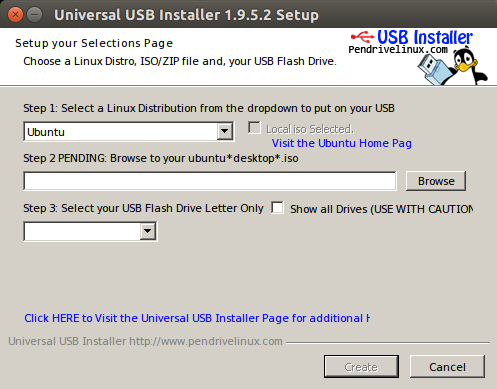
\includegraphics[width=\linewidth]{images/instalacja_nagrywanie_obrazu.png}
\end{wrapfigure}
\noindent Jeżeli chcesz użyć pendriva jako nośnika instalacyjnego to upewnij się iż ma on przynajmniej 1 gigabajt pojemności. W przeciwnym wypadku instalator nie zmiejści na nim. Jeżeli masz już przygotowany pendrive, wykonaj co następuje:
\begin{enumerate}
%TODO dla tej listy użyć włąsnych znaczników (label) przypominających te użyte na obrazkach.
\item Pobierz program \href{http://www.pendrivelinux.com/downloads/Universal-USB-Installer/Universal-USB-Installer-1.9.5.2.exe}{Universal USB Installer}.
\item Uruchom pobrany plik.
\item Zaakecptuj umowę licencyjną.
\item Podłącz do komputera pendrive, który ma użyty jako nośnik.
\item Z tej listy wybierz Ubuntu.
\item Kliknij na przycisk Browse i wskaż pobrany wcześniej obraz instalatora Ubuntu.
\item Z tej listy wybierz wczesniej podłączony pendrive.\\
\textbf{UWAGA: Wszystkie dane na nim zostaną skasowane!}
\item Kliknij przycisk CREATE.
\item Poczekaj na zakończenie operacji.
\end{enumerate}
\clearpage
\subsubsection{System Windows 7 / 8, nagrywanie na płytę DVD}
%TODO zweryfikować, czy windows 8 też to ma
\begin{wrapfigure}{r}{0.5\textwidth}
		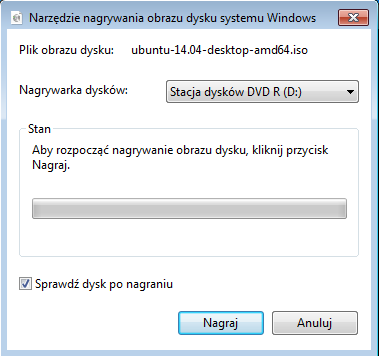
\includegraphics[width=\linewidth]{images/instalacja_nagrywanie_obrazu_DVD.png}
\end{wrapfigure}
Systemy operacyjne Windows 7 i 8 mają wbudowane narzędzie do wypalania plików .iso na płytach. Kliknij prawym przyciskiem myszy na pobrany obraz instalatora Ubuntu, wybierz opcję "Otwórz w" a następnie "Windows Disc Image Burner".
\begin{enumerate}
%TODO dla tej listy użyć włąsnych znaczników (label) przypominających te użyte na obrazkach.
%TODO jak to się po polsku nazywa?
\item Z tej listy wybierz swoją nagrywarkę.
\item Włóż czystą płytę DVD na wybranego napędu.
\item Upewnij się, że zaznaczone jest pole "Zweryfikuj dysk po nagraniu"
\item Kliknij na przycisk \textbf{Nagraj}
\end{enumerate}
\clearpage
\subsubsection{System Windows XP i inne starsze wersje, nagrywanie na płytę DVD}
\begin{wrapfigure}{R}{0.5\linewidth}
		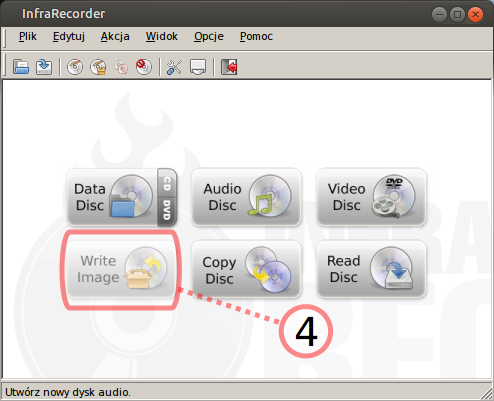
\includegraphics[width=\linewidth]{images/instalacja_nagrywanie_obrazu_DVD_winXP.png}
\end{wrapfigure}
Starsze wersje systemu Windows nie mają wbudowanej możliwości nagrywania płyt DVD. Potrzebne będzie do tego osobne narzędzie, program służący do wypalania płyt. Obsługa tych programów jest bardzo podobna: należy wybrać opcję \emph{Nagrywanie obrazu na płytę}. Koniecznie nagrywaj z wykorzystaniem tej opcji, gdyż inne (np.\emph{Nagrywanie płyty z danymi} lub \emph{Tworzenie kopi zapasowej}) utworzy dysk, którego twój komputer nie będzie potem wstanie uruchomić. Dla przykładu posłużymy się programem Infra Recorder.

\begin{enumerate}
\item Pobierz i zainstaluj program \href{http://infrarecorder.org/?page_id=5}{Infra Recorder}.
\item Uruchom nowozainstalowany program.
\item Włóż czystą płytę DVD do nagrywarki.
\item W programie Infra Recorder wybierz opcję \textbf{Write Image}.
\item Wybierz pobrany wcześniej obraz instalatora Ubuntu.
\item Kliknij na przycisk \textbf{OK}.
\end{enumerate}
\clearpage











\end{document}
